% !TeX root = ../libro.tex
% !TeX encoding = utf8
%
%*******************************************************
% Introducción
%*******************************************************

% \manualmark
% \markboth{\textsc{Introducción}}{\textsc{Introducción}}

\chapter{Introducción}
La revolución digital marcó el inicio de lo que hoy en día se conoce como la \emph{Era de la información}. No es de extrañar que vivamos rodeados de dispositivos que estén constantemente transmitiéndose información entre ellos, seamos o no conscientes de qué información mandan, cómo, a quién y para qué. \\

%No sólo estamos tan rodeados de tantos dispositivos sino que la evolución transmitida no sólo ha evolucionado sino que seguirá haciéndolo. Ya no se conocen únicamente sino que también se es capaz de extraer detalles cada vez más complejos de los datos compartidos.\\

Entre todos estos datos transmitidos tiene una gran relevancia el contenido multimedia. No se trata de conocer sólo el quién, el cuándo y el a dónde, entre otras cuestiones, sino también \emph{qué}. Cuando se habla de conocer qué se transmite no nos referimos a la imagen RGB en sí, sino al contenido propio de la imagen. ¿La imagen transmitida es una foto o un dibujo? ¿Qué o quiénes aparecen en la imagen? ¿Con qué cantidad? ¿Representa una escena feliz?\\

Son muchas las preguntas que pueden nacer a través del contenido que representa una única imagen y estas se podrían responder fácilmente con una persona que, de forma subjetiva, anotase una respuesta para cada una de ellas. Pero, ¿y si se extendiera a miles de millones de imágenes?, ¿y si no sólo quisiéramos conocer el contenido de la imagen, sino también la relación existente entre diferentes imágenes?\\

Para responder a estas preguntas, existen diferentes métodos que extraen la información deseada, algunos siendo más especializados que otros para algunas cuestiones concretas. En particular, en este proyecto se le da especial atención a las redes neuronales convolucionadas como método de extracción de información. Esta, será utilizada a través de un sistema de recuperación de información basada en su contenido (CBIR) para comparar la relación existente entre las diferentes imágenes.\\

Un ejemplo de sistema funcional que implementa una recuperación de imágenes basadas en su contenido lo podemos encontrar en \href{https://www.google.es/imghp?hl=es&authuser=0&ogbl}{\emph{Google Image}}. Dependiendo de la imagen, este buscador será capaz de proporcionar la misma imagen en diferentes dimensiones, las webs en en las que han sido utilizadas u otras imágenes similares. No sólo eso, sino que, dependiendo de en qué webs haya sido utilizada, realiza un etiquetado de posibles términos capaces de describir la imagen.\\

Sin embargo, debido a la gran cantidad de información que analiza y compara el ejemplo mencionado, los resultados que muestra no son siempre los deseados para la búsqueda y recuperación de imágenes. ¿A qué nos referimos con que no son los deseados? En este contexto, se quieren obtener imágenes similares o relacionadas con la imagen original y no imágenes pertenecientes a webs con contenido similar.\\

Es decir, si estamos buscando una imagen con un ``autobús'' central y en grande, se desearán obtener más imágenes que posean autobuses y no la misma imagen repetida en diferentes enlaces. De la misma forma, si la imagen que utilizamos para la búsqueda se trata de un ``puerto'', querremos obtener imágenes de diferentes puertos \autoref{fig:puerto-autobus}.\\

\begin{figure}[h!]
  \centering
  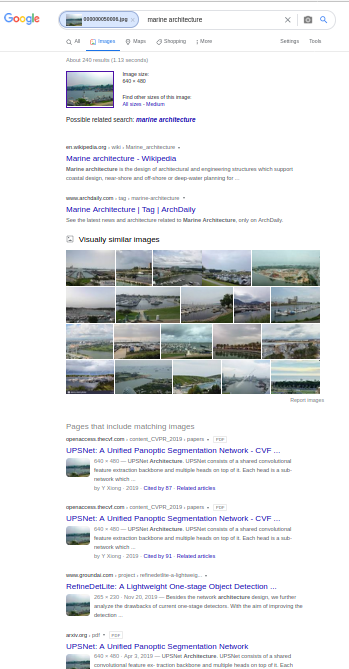
\includegraphics[width=0.48\textwidth]{puerto}
  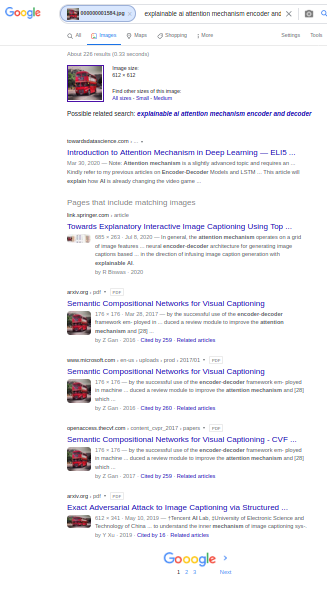
\includegraphics[width=0.48\textwidth]{bus}
  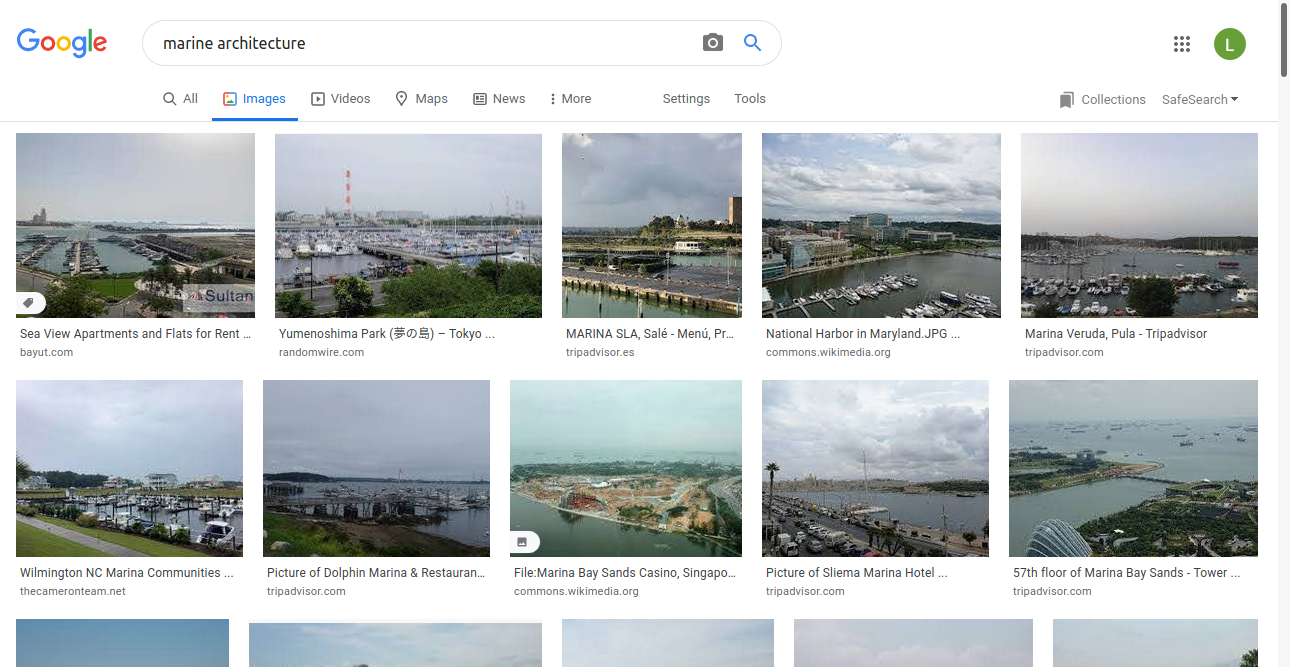
\includegraphics[width=0.48\textwidth]{puerto-}
  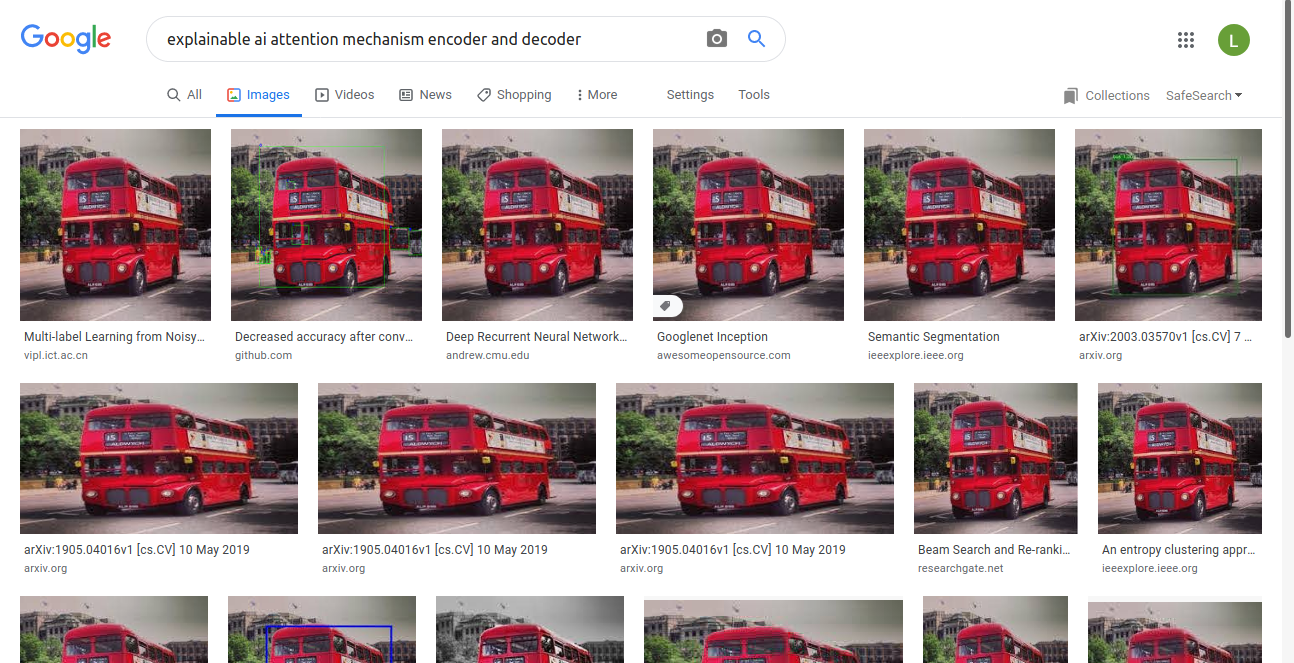
\includegraphics[width=0.48\textwidth]{bus-}
  \caption{Resultados de búsqueda de imágenes utilizando la funcionalidad de \emph{Google}. A la izquierda, se puede ver el resultado de la búsqueda de un puerto y, a la derecha, la búsqueda de un autobús. Nótese que con el puerto sí aparecen imágenes similares mientras que con el autobús únicamente aparecen enlaces que poseen la misma imagen o versiones redimensionadas de esta.}
  \label{fig:puerto-autobus}
\end{figure}

\newpage
Cuando Google realiza un etiquetado de la imagen, este lo realiza de forma global y sin tener en cuenta la posibilidad de la localización de los distintos objetos. En este proyecto se estará realizando un etiquetado local de las regiones de la imagen y se podrá realizar una comparación dependiendo de la posición relativa de los objetos identificados.\\

Para ello, se implementarán una serie de bases de datos de imágenes y será en estas en las que podrán realizar las búsquedas. Además, como funcionalidad extra, se podrán seleccionar los criterios de comparación utilizados para averiguar cómo de parecidas serán las distintas imágenes de la base de datos con la imagen que estaremos utilizando en la consulta.\\

Es decir, no sólo le damos más importancia a la propia imagen que queremos utilizar como consulta, sino que, además, se permite la adición de criterios de búsqueda más específicos o con mayor libertad, dependiendo de lo que se desee en cada momento.\\

Para desarrollar la extracción de características de una imagen utilizaremos redes neuronales convolucionadas, pero no utilizaremos una red neuronal ya existente. Si bien sí comentaremos el estado del arte, sino que se analizará una posible mejora planteada en \cite{DBLP:journals/corr/abs-1711-07971} basada en desarrollo de bloques que utilicen operaciones capaces de extraer la relación existente entre todas las posiciones de la imagen, y no únicamente en un entorno como sucede con la operación de convolución.\\

\section*{Objetivos}
Dicho esto, los objetivos marcados para el trabajo serán:\\
\begin{enumerate}
\item Estudiar y demostrar que las redes neuronales son aproximadores universales.
\item Estudiar el concepto de operación no local \cite{DBLP:journals/corr/abs-1711-07971}.
\item Comparar la utilidad de bloques que utilicen el operador no local con su no utilización o la utilización de convoluciones.
\item Desarrollar un sistema de recuperación de información basado en su contenido.
\item Utilizar la información extraída a través de una red neuronal en el sistema implementado.
\item Implementar la comparación de la información extraída.
\end{enumerate}

\section*{Organización de la memoria}
Respecto a la organización de la memoria, esta estará organizada en cuatro partes fundamentales.\\

En la primera parte se introducirán los conceptos teóricos y se introducirán una serie teoremas que permitirán sentar las bases de los experimentos que se realizarán en las demás partes.\\

Se comenzará con una introducción amigable a la utilización de redes neuronales, mostrando su estructura de forma genérica y mencionando algunos de los algoritmos y funciones más sencillas que pueden llegar a ser utilizadas. En particular, se hablará sobre las funciones de activación, de pérdida y de medida más comunes. Se continuará mostrando versiones sencillas de los algoritmos de propagación hacia delante y hacia atrás, además de los algoritmos de aprendizaje de descenso del gradiente estocástico y \emph{Adam}.\\

Será en la segunda sección donde nos detendremos a hablar sobre los teoremas de aproximación universal. Aquí mencionaremos varios teoremas que, cada uno de ellos bajo diferentes condiciones de partida, buscan demostrar que una red neuronal es capaz de aproximar cualquier función. Tendremos dividida esta sección de acuerdo a qué parámetro dejen como indeterminado en los diferentes teoremas, es decir, tendremos los casos de anchura indeterminada y de altura indeterminada.\\

En la tercera sección explicaremos lo que son las redes neuronales convolucionadas, así como las capas más importantes para este tipo de redes. Estás serán las capas que implementen operaciones de convolución y aquellas que agrupen o condensen la información obtenida, las llamadas capas \emph{pooling}.\\

La primera parte finalizará con la introducción del concepto de operador no local. La utilidad de este operador será que, conforme aumenta el tamaño de la imagen, podremos encontrar más regiones similares. Es decir, si tenemos una imagen con una naranja, cuanto más grande sea la imagen, más posibilidades tendremos de encontrar otra naranja. Para poder utilizar con propiedad este operador, se introducirán una serie de conceptos relacionados con los procesos estocásticos que permitirán enunciar un teorema que demostrará la consistencia de dicho operador, cuya demostración, debido a su extensión, será referencia al trabajo original.\\

La segunda parte estará centrada en la segmentación semántica de imágenes. Esta comenzará comentando las familias más importantes del estado del arte actual de la segmentación semántica y de la instanciación de objetos en imágenes. Concretamente, se hablarán de las familia RCNN y de las distintas versiones de YOLO.\\

Seguidamente, se hablará de lo que son las \emph{non-local neural networks}, un tipo de redes neuronales que siguen una arquitectura ascendente y descendente para extraer las características de nuestros datos de entrada a distintos niveles de profundidad de la red. Estas redes implementan bloques que utilizan lo que hemos definido como operador no local y buscamos comprobar en una serie de ejemplos concretos cómo de bien o mal funcionan estos bloques.\\

Para ello, se diseñaran una serie de redes neuronales convolucionadas con pequeñas diferencias entre sí, que serán analizadas para comprobar cómo difiere el comportamiento de la red ante estos cambios.\\

%En la siguiente parte hablará de las redes más importantes en el estado de arte actual antes de centrarnos en el diseño de una red neuronal con una estructura sencilla pero que permita, a través de pequeñas modificaciones, la comparación entre las diversas posibilidades que se plantearán. Se analizarán los resultados obtenidos y se obtendrán conclusiones de acuerdo al ejemplo concreto utilizado.\\

En la tercera parte se tendrá el diseño y desarrollo del sistema de recuperación de imágenes implementando, utilizando para ello la biblioteca \emph{Java Multimedia Retrieval} \cite{JMR}. Concretamente se diseñará e implementará un descriptor que reunirá información de las imágenes a través del uso de las redes neuronales anteriormente implementadas y junto con un comparador de objetos descriptores para poder ordenar las imágenes de dependiendo de su similitud con la imagen consultada. También se tendrá el manual de usuario y se realizarán una serie de pruebas para mostrar el comportamiento del prototipo ante diferentes parámetros.\\

Finalmente, tendremos una serie de conclusiones obtenidas a lo largo del proyecto y se comentarán algunos posibles trabajos futuros.
\endinput
